% !tex-engine = luatex
\documentclass{lukereport}

%%%
% Next packages are for the template examples and can be removed.
\usepackage{lipsum}
%%%

%% dev, to be moved to class-file
\usepackage{multirow, tabularx}

% Title Page
\title{Report title to be written here}
%\subtitle{Report specifier (if any)}
\author{Firstname Lastname}


\begin{document}
\maketitle

\begin{abstract}
\lipsum[2-3]
\end{abstract}

%\newpage
\setcounter{tocdepth}{2}
%\tableofcontents

%\newpage


\chapter{Heading 1}

\lipsum[1]

\section{Heading 2 (TOC included)}

\lipsum[2]

\subsection{Heading 3 (TOC included)}
\begin{figure}[!hb]
	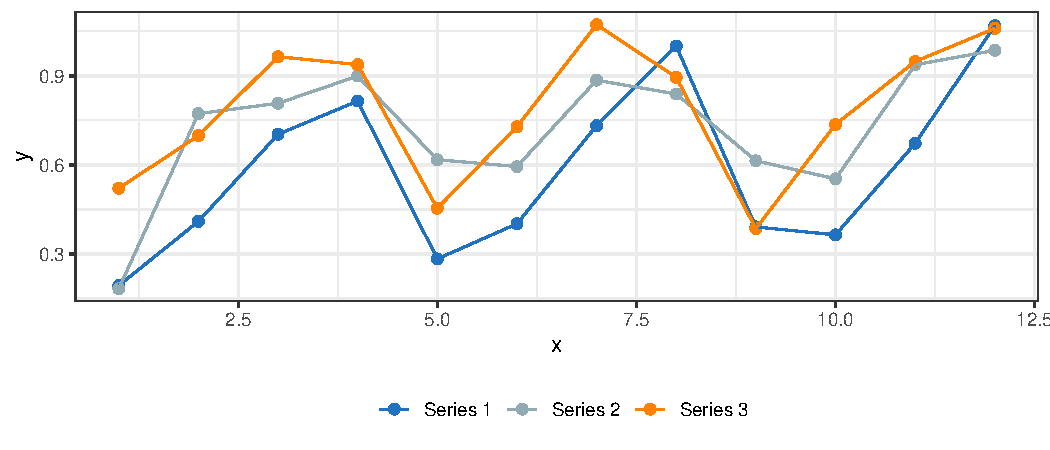
\includegraphics[width=.8\linewidth]{fig_ex1}
	\caption[short figure caption]{Long figure caption.}
	\label{fig:figex1}
\end{figure}

\lipsum[4]

\subsubsection{Heading 4 (TOC not included)}


\lipsum[6] See Figure \ref{fig:figex1}.


\chapter{Heading 1}

\lipsum[1]

\section{Heading 2 (TOC included)}

\lipsum[2]

\subsection{Heading 3 (TOC included)}
\lipsum[4]

\subsubsection{Heading 4 (TOC not included)}
\lipsum[6]



% \begin{table}
% 	\label{tab:basic}\caption{Basic table.}
% 	
% 	\begin{tabularx}{\textwidth}{l|c|c|c|c|}
% 		\hline
% 		\multirow{2}{*}{Mäkinen ym. (2006), ensiharvennus} &  
% 		\multicolumn{2}{c}{Mänty}  &  \multicolumn{2}{c}{Kuusi} \\
% 		%\hline
% 		&  Valikoiva harvennus& Käytävä\-harvennus  &  Valikoiva harvennus & 
% 		Käytävä\-harvennus\\
% 		\hline
% Kokonaispuuusto\footnote{footnote 1}, $m^3/ha$		&  &  &  &\\
% 		\hline
% Kuitupuu		&  &  &  &\\
% 		\hline
% Yhteensä		&  &  &  &\\
% 		\hline
% Keskimääräinen tilavuuskasvu, $m^3/ha/v$		&  &  &  & \\
% 		\hline
% 	\end{tabularx}
% 	
% \end{table}



\end{document}      
